\chapter{Topology: What Counts as the Same Shape in Modelling Clay?}

\section{A Map That Does Not Look Like a Map}

You have probably travelled by underground and certainly seen its colourful route map: horizontal and vertical lines, evenly spaced dots, and tidy corners. Overlay it on a real city map and almost nothing matches. Stations two centimetres apart on paper may be five kilometres apart; a perfectly straight line on the diagram may twist repeatedly underground. In lengths, angles, and areas, this map tells lies everywhere.

Strangely, passengers do not get lost because of it. When draughtsman Harry Beck drew the first such London Underground map in 1933, the company initially hesitated: would passengers accept something so unrealistic? In practice, it proved so useful that underground systems worldwide copied it. Why? Passengers care about three things: their current station, their destination, and where to change. The tunnels' precise turns, or whether stations are eight hundred or twelve hundred metres apart, do not matter. Beck saw this clearly: he discarded distracting real-world detail and retained only **what connects to what**.

This raises a deep question: a map can be distorted beyond recognition yet still answer certain questions correctly. Which properties of a figure survive arbitrary stretching, bending, and compression? Which vanish at a gentle squeeze? The study of the former is called **topology**, famously nicknamed rubber-sheet geometry. To a topologist, figures are made of unbreakable modelling clay: knead them however you like, but do not tear them or glue separate parts together. The properties that remain unchanged are the ``true shape'' topology studies.

In this chapter we become clay modellers. We will see how a three-hundred-year-old walking puzzle helped create the subject; why coffee cups and doughnuts look identical to topologists; why a strip of paper loses its front and back after a half-twist; and how these playful ideas serve networks, maps, and robots.

\section{Seven Bridges and an Impossible Walk}

Our story begins in a real city. In eighteenth-century Konigsberg, now Kaliningrad in Russia, a river crossed the town, with two islands and seven bridges linking them to its banks. A favourite leisure puzzle reportedly prompted years of tavern debate:

\begin{quote}
Can you set out from home, cross each of the seven bridges exactly once, and finally return home?
\end{quote}

Before reading on, guess: possible or impossible? Many instinctively say yes: enough attempts should find a route. Others say no but cannot explain why. That is the puzzle's charm: it sounds like a riddle, yet nobody can supply a convincing answer. Clever townspeople repeatedly trace routes on maps, always getting stuck at the last bridge or two: either crossing one twice or reaching an island with no unused bridge left.

Trying indefinitely has a fatal weakness: ten thousand failures do not prove the ten-thousand-and-first attempt cannot succeed. Proving impossibility requires a new viewpoint, not more attempts. In 1736, Euler, then living in St Petersburg, heard the puzzle. His first move seemed remarkably unmathematical: he threw away the map.

\section{What Remains After Scrunching Up the Map?}

Euler reasoned that the size of the banks, the islands' shapes, bridge lengths, and road bends were irrelevant. The walker only experiences being on a piece of land and crossing a bridge to another piece. He shrank each of the four land areas---two banks and two islands---to a point, and each bridge to a line connecting points. The result was an ugly little diagram, four points and seven lines, that a primary-school pupil could draw in seconds:

\begin{center}
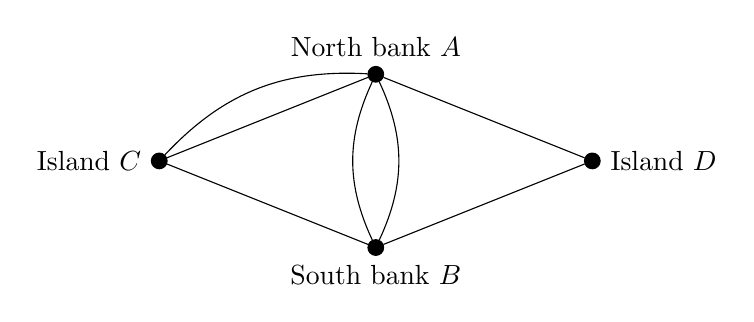
\begin{tikzpicture}[scale=1.1]
  \node[circle,draw,fill=black,inner sep=2pt,label=above:{North bank $A$}] (A) at (0,2) {};
  \node[circle,draw,fill=black,inner sep=2pt,label=below:{South bank $B$}] (B) at (0,0) {};
  \node[circle,draw,fill=black,inner sep=2pt,label=left:{Island $C$}] (C) at (-2.5,1) {};
  \node[circle,draw,fill=black,inner sep=2pt,label=right:{Island $D$}] (D) at (2.5,1) {};
  \draw (A) to[bend left=25] (B);
  \draw (A) to[bend right=25] (B);
  \draw (C) -- (A);
  \draw (C) to[bend left=25] (A);
  \draw (C) -- (B);
  \draw (D) -- (A);
  \draw (D) -- (B);
\end{tikzpicture}
\end{center}

The original question becomes: can we start at a point, **trace every line exactly once**, and return to the start? This is the familiar childhood one-stroke drawing puzzle!

Notice this remarkable step. Before solving the original problem, Euler established that it and the drawing puzzle are **the same problem**. He compressed the map into a little tangle of threads, discarding lengths, areas, and shapes without losing any information the question needed. Keeping only connections is a basic topological skill. The more we discard, the clearer the remaining structure becomes.

Before continuing, we need official names for these points and lines so we can speak precisely.

\begin{dingyi}[Graphs, vertices, edges, and degrees]
A collection of points, called \textbf{vertices}, and connecting lines, called \textbf{edges}, forms a \textbf{graph}. The number of edges meeting a vertex is its \textbf{degree}. Vertices of odd degree are \textbf{odd vertices}; those of even degree are \textbf{even vertices}. A graph is \textbf{connected} if every vertex can be reached from any other by following edges.
\end{dingyi}

Count the degrees in the seven-bridge diagram: $A$ meets $5$ edges, $B$ meets $3$, $C$ meets $3$, and $D$ meets $3$. All four vertices are odd. Remember this: it will solve the mystery.

\begin{shuyu}{Topological equivalence (homeomorphism)}
Intuition: If two clay figures can be transformed into one another by continuous stretching, bending, and compression, without tearing or gluing, they have the same shape.\\
Formal definition: Two figures are \textbf{homeomorphic} if there is a continuous one-to-one correspondence between them whose inverse is also continuous.\\
Example: A circle and a square are homeomorphic: stretch the circle like a rubber band into a square frame. A circle and a figure eight are not: the figure eight's central crossing cannot be separated.
\end{shuyu}

\section{Solving the Mystery: Count the Odd Junctions}

Now solve the one-stroke puzzle. Imagine following the graph with a pen. At an intermediate vertex, you must enter along one edge and leave along another, using incident edges in pairs. A vertex that is neither the start nor the finish must therefore have its edges paired as entrances and exits: its degree must be even.

What about the endpoints? If the walk returns to its start, the initial departure and final arrival also pair up, as do intermediate visits, so the starting vertex is even too. There can be no odd vertices anywhere. If return is not required, the start has one extra departure and the finish one extra arrival. These two may be odd, but no others. This is Euler's discovery:

\begin{dingli}[Euler's one-stroke theorem, 1736]
For a connected graph:
\begin{enumerate}
  \item A route using every edge exactly once and returning to its start exists if and only if there are \textbf{no} odd vertices.
  \item A route using every edge exactly once, without necessarily returning to its start, exists if and only if there are \textbf{exactly two} odd vertices, which must be its endpoints.
\end{enumerate}
\end{dingli}

\begin{proof}
First prove necessity. Each intermediate visit uses two edges, one entering and one leaving, so all vertices other than the endpoints are even. For a closed route, the starting vertex's initial and final edges also pair up, making it even; there are no odd vertices. For an open route, the start and finish each have one unpaired edge and are exactly the two odd vertices.

Now prove sufficiency, beginning with no odd vertices. Start anywhere and follow unused edges arbitrarily. Because edges at every vertex pair up, entering any vertex other than the start always leaves an unused exit. The only place you can get stuck is therefore the start. Continue until stuck: you have a closed route. If unused edges remain, connectivity guarantees that some vertex on this route meets an unused edge. Start another arbitrary walk there; the same reasoning brings it back to that vertex. Insert this new circuit into the original route to make a longer one. Repeat until every edge is used. With exactly two odd vertices, start at one and eventually get stuck at the other, then insert remaining circuits in the same way.
\end{proof}

Return to the bridges: all four vertices are odd, giving $4$, neither $0$ nor $2$. The walk **does not exist**: not merely undiscovered, but impossible to discover. Without walking a step, Euler counted bridges at each junction and settled years of argument. Reportedly, an eighth bridge later left two odd vertices, finally permitting a walk across every bridge, though not back home. Mathematics predicted possibility and engineering followed: an ironically fitting sequel.

\begin{toolbox}
Our new tools so far:
\begin{itemize}
  \item \textbf{Compression}: Turn a map into points and lines, retaining only connections.
  \item \textbf{Graphs} (vertices, edges, degrees) and \textbf{connectivity}: Minimal language for what connects to what.
  \item \textbf{Parity pairing}: Entrances and exits pair up; parity drives the argument.
  \item \textbf{Homeomorphism}: The criterion for sameness of shape in modelling clay.
\end{itemize}
\end{toolbox}

\section{Classifying Letters: What Is a Topological Property?}

With homeomorphism as our measuring stick, try a classification game. Imagine printed capital letters as thin clay lines: A, B, C, D, E, and so on. Which have the same shape?

C, I, J, L, M, N, S, U, V, W, and Z form one class: each is a line that can be straightened into a segment. A, D, O, P, Q, and R form another: each has **one hole**, whether triangular as in A or round as in O. B stands alone with **two holes**. E, F, T, and Y have no holes but **one three-way junction**. K and X have a four-way junction. H is special, with two three-way junctions.

What does this game tell us about topology's interests? The classification uses only a few properties:

\begin{itemize}
  \item \textbf{Connectivity}: Is the figure one piece or several? Whether the dot on a lowercase i connects to its stem is a connectivity question.
  \item \textbf{Number of holes}: How many independent loops cannot be bypassed?
  \item \textbf{Junctions and endpoints}: Where do lines branch, and where do they terminate?
  \item \textbf{Boundary}: Does the figure have an edge, and how many boundary components are there?
\end{itemize}

Lengths, angles, areas, and curvature are absent. Topologists famously joke that they cannot distinguish a coffee cup from a doughnut. Imagine a clay cup with a handle: press in and round its body, leaving the handle as a ring, and it becomes a doughnut. Nothing is torn or glued; the handle's hole becomes exactly the doughnut's hole. A doughnut, however, can never become a **sphere without a hole**. Every rubber loop on a sphere can shrink to a point, while a loop around the doughnut can get caught on its ring. Hole count is the first checkpoint separating shapes into species.

\begin{fanli}
``These figures look very different, so they are topologically different'' is false: a circle and a square look different but are homeomorphic. Conversely, equal area does not imply topological sameness. A disc and an annulus can have equal areas, yet one has no hole and the other has one; clay deformation cannot create that hole. Homeomorphism concerns continuous deformation, not appearance or size.
\end{fanli}

\section{A Number That Counts Holes: The Euler Characteristic}

Holes are useful, but counting them can be ambiguous: how many holes does a piece of cheese pierced three times have? Mathematicians need a mechanical, uncontentious measure of how a shape winds around. The method is surprisingly simple: cut the figure into pieces, count three kinds of components, and add and subtract.

Start with convex polyhedra. A cube has $8$ vertices, $12$ edges, and $6$ faces:
\[
V - E + F = 8 - 12 + 6 = 2.
\]
A regular tetrahedron has $V=4$, $E=6$, and $F=4$, giving $4-6+4=2$. A regular dodecahedron has $V=20$, $E=30$, and $F=12$, again giving $20-30+12=2$. Curious, isn't it? Wildly different component counts always yield $2$. Euler---yes, him again, appearing in nearly every corner of mathematics---proved this was no coincidence:

\begin{dingli}[Euler's polyhedron formula]
Every polyhedron continuously deformable into a sphere, or connected graph drawn on a sphere, satisfies
\[
V - E + F = 2,
\]
where $V$, $E$, and $F$ count vertices, edges, and faces respectively.
\end{dingli}

\begin{proof}[Proof sketch]
Imagine the polyhedron as a hollow rubber balloon. Remove one face and flatten the rest onto a table, producing a connected graph of vertices and edges. It divides the plane into regions, $1$ fewer than the original face count, since the removed face becomes the unbounded exterior. We need to prove $V-E+F_{\text{regions}}=1$ for the flattened graph. Perform two demolition operations. If a cycle remains, delete one of its edges: $E$ decreases by $1$, and the regions on its two sides merge, decreasing $F_{\text{regions}}$ by $1$, so $V-E+F_{\text{regions}}$ is unchanged. Once no cycles remain, the graph is a tree. Remove an endpoint and its incident edge: $V$ decreases by $1$ and $E$ by $1$, again preserving $V-E+F_{\text{regions}}$. Eventually only a lone vertex remains: $V=1$, $E=0$, $F_{\text{regions}}=0$, giving $1$. Since neither operation changed the value, the original planar graph also gives $1$, and restoring the polyhedron gives $2$.
\end{proof}

The number $V-E+F$ is the \textbf{Euler characteristic}, usually denoted by the Greek letter $\chi$. Remarkably, however the surface is subdivided---large pieces or small, straight edges or curved---the value of $\chi$ remains the same. It is the surface's fingerprint.

Fingerprints distinguish species. Repeat the game on a doughnut, or torus: draw a connected graph dividing it into regions, and obtain $V-E+F=0$. A two-holed double torus, like two joined swimming rings, gives $-2$. Each added hole lowers $\chi$ by $2$. Writing $g$ for the hole count, mathematically called the \textbf{genus}, we have
\[
\chi = 2 - 2g.
\]
A sphere has $g=0$, $\chi=2$; a doughnut $g=1$, $\chi=0$; a double torus $g=2$, $\chi=-2$. The vague task of counting holes becomes arithmetic with an agreed answer: grid the surface, count, and subtract. A coffee cup can become a doughnut because both have $\chi$ equal to $0$; neither becomes a sphere because $\chi=0$ never equals $\chi=2$.

\begin{shuyu}{Euler characteristic}
Intuition: Conduct a surface census. Vertices minus edges plus faces gives an identification number unchanged by continuous deformation.\\
Formal definition: Subdivide a surface into $V$ vertices, $E$ edges, and $F$ faces; $\chi = V - E + F$, independently of the subdivision.\\
Example: A cube gives $8-12+6=2$, placing it with the sphere; a torus grid gives $0$, smaller by $2$, corresponding exactly to its extra hole.
\end{shuyu}

\section{A Half-Twisted World: The Mobius Strip and Klein Bottle}

Our clay game has so far kept an unspoken rule: surfaces have an inside and an outside. A balloon has inner and outer walls; paper has front and back. In 1858, Mobius discovered a surface with only **one side**, absurdly easy to make: take a long paper strip, twist one end halfway around, and join it to the other.

Try it; the experiment below will guide you. Draw a coloured line along the strip's centre without lifting the pen. Eventually you return to your starting point, having marked ``both sides'': there is no other side! Cut along the centre line, and instead of the expected two rings, you obtain one longer ring with a full twist. An ant can crawl over the entire Mobius strip without crossing an edge.

\begin{shiyan}
Cut a scrap-paper strip about $3$ centimetres wide and $25$ centimetres long.
\begin{enumerate}
  \item Join the ends directly to make an ordinary ring. Draw around its centre line: only one side is marked. Cut along that line and the ring separates into two rings.
  \item Make another strip, twisting one end halfway around before joining it. Draw the centre line: the marks now magically cover the whole strip. Cut along the line and count the twists in the resulting ring.
  \item Join another strip after a full twist, $360^{\circ}$. Repeat the drawing and cutting. How does this differ from the previous two?
  \item Record the number of resulting rings and their twists after starting with $0$, half, one, and one-and-a-half turns. Can you guess a pattern?
\end{enumerate}
\end{shiyan}

A Mobius strip also has one **boundary**: before cutting, its long paper edge surprisingly forms a single connected line. Mathematicians then asked whether a closed surface could have one side and no boundary at all. Yes: the \textbf{Klein bottle}. Imagine making a hole in a bottle's base, lengthening its neck, bending it back through the bottle wall, and joining it to the hole. Inside and outside become one surface: walking along the wall takes you from exterior to interior without crossing any edge. An ant can explore the entire Klein bottle.

There is a fact we must admit: a Klein bottle **cannot be built** in our three-dimensional space. The description required passing through the bottle wall. In three dimensions, the neck must penetrate the body to reach the base, violating the clay game's no-puncturing rule. Only in four dimensions can it detour through a fourth direction without touching the wall. Glass ``Klein bottles'' sold as ornaments all self-intersect: they are three-dimensional projections of a four-dimensional resident, just as a doughnut's shadow on a wall may contain crossings. Mobius strips show that the number of sides is not a given; Klein bottles show that some shapes do not fit our world, yet mathematics describes them precisely.

\begin{lianjie}
Remember turning squares, rotations, and reflections into a symmetry operation table? There we upgraded ``looks the same'' to ``has the same structure''. This chapter makes the same upgrade with a different measuring stick. Chapter 6 asked which motions leave a figure unchanged; here we ask which deformations leave properties unchanged. Our graphs speak the same language as Chapter 14's graph theory: the bridges problem is a shared birth certificate for graph theory and topology. Next chapter, see what happens when rulers and protractors replace the modelling clay.
\end{lianjie}

\section{Another Perspective: Networks, Maps, and Robots}

Topology sounds like clay play and paper cutting, but preserving connections while discarding detail is a fundamental principle of the modern world.

\textbf{Networks.} The internet has hundreds of millions of devices, transport networks thousands of junctions, and power grids countless nodes. Engineers often ask first not how long a cable is, but topological questions: is the network connected? Will losing a node split it in two? How large will the pieces be? This is the same thinking as asking how many pieces a figure has. Social networks' six degrees of separation---roughly six friendship links between any two people on average---describe surprisingly tight connections in enormous networks.

\textbf{Maps.} What is the minimum number of colours needed for a world map so neighbouring countries differ? The question depends only on shared borders, not countries' areas, shapes, or coastline curves: it is purely topological. For over a century, people conjectured that four colours suffice, the famous four-colour conjecture. In 1976, mathematicians reduced it to checking over a thousand basic configurations and completed the proof by computer. This became the first major computer-assisted theorem. Some mathematicians still debate whether a proof no individual can check by hand counts as a proof.

\textbf{Robots.} A robotic arm has several joints, each rotating through an angle. Every pose corresponds to a point in a configuration space formed from those angles. Planning motion means finding a continuous collision-free path through that space. Its topology is intriguing: a joint permitting full rotation contributes a circle; two independently rotating joints contribute a torus, our doughnut again! Robot engineers effectively plan routes on doughnuts, spheres, and stranger surfaces. Many obstacles that no turn seems to bypass are fundamentally holes in configuration space.

\begin{zhu}
In these applications, topology answers questions of possibility: can things connect, can a route go around, can four colours suffice? Speed, length, and cost require bringing back lengths and angles and calling on other branches of mathematics. Distinguishing ``possible or impossible'' from ``better or worse'' is a first step in problem-solving.
\end{zhu}

\begin{pandeng}
For further climbing, remember these keywords: \textbf{fundamental group}, making non-shrinkable loops into an algebraic structure and hole counts into rigorous theorems; \textbf{homology}, a distant relative of the Euler characteristic that counts holes of any dimension; \textbf{knot theory}, studying when knots in three-dimensional space can be undone, from shoelaces to DNA; and the \textbf{Poincare conjecture}, the three-dimensional version of ``a closed shape without holes must be a sphere'', proved only in 2003 and the first Millennium Prize Problem to be solved.
\end{pandeng}

\section*{Questions to Think About}

\textbf{Observation}

\begin{sikao}
  \item Treat the digits $0$ to $9$ as thin clay lines, handwritten without crossings, and classify their topological shapes. Which belong together? \textbf{Hint}: first count holes and endpoints.
  \item Lay an unbuttoned long-sleeved shirt flat. Topologically, it resembles a disc with how many holes? \textbf{Hint}: count all the exits once a body is inside, and consider how many holes each exit represents.
\end{sikao}

\textbf{Proof}

\begin{sikao}
  \item Prove that every graph has an even number of odd vertices. \textbf{Hint}: when adding every vertex's degree, how many times is each edge counted? Is the total odd or even?
  \item Check $V-E+F$ on a sphere with a latitude--longitude grid, say $4$ meridians and $2$ latitude circles, one being the equator. Count the poles as vertices. Count vertices, edges, and regions to verify Euler's formula. \textbf{Hint}: decide how meridian intersections at the poles count and how many pieces each latitude circle is cut into.
\end{sikao}

\textbf{Challenge}

\begin{sikao}
  \item What is the largest number of pairwise adjacent regions on a doughnut, every pair sharing a boundary? On a plane it is at most $4$, one source of the four in the four-colour theorem; a doughnut allows more. \textbf{Hint}: the answer is $7$. First try drawing $5$ pairwise adjacent regions, then exploit routes around the ring to fit two more.
  \item Join two Mobius strips along their boundaries. Which surface from this chapter results? \textbf{Hint}: mentally unfold one strip into a ring-shaped band; consider whether a Klein bottle can be cut into two halves along some line.
\end{sikao}

\section*{The Door to the Next Chapter}

We have enjoyed considerable freedom: discard lengths, angles, and areas, and call a figure unchanged as long as its connections and holes remain. In the clay world, a sphere and a potato are the same kind of thing; a teacup and a doughnut are indistinguishable.

Earth's inhabitants will object that Earth is not a potato. Navigation software needs distances; pilots need to know why Beijing--New York flights first head north rather than straight east along a latitude circle. Such questions immediately require what we discarded: length, angle, and curvature. Spherical triangles have angle sums greater than $180^{\circ}$, and straight lines on a torus can wind around themselves. Topology sees none of this, because a squeeze of clay changes it all.

Replace the clay with a firmer curved surface, allowing travel across it but no stretching. The straightest route, shortest distance, and degree of bending then need a new language. How does a surface locally resemble a plane? Can a blindfolded ant tell from underfoot measurements whether it lives on a sphere or a plane? Next we enter differential geometry: distances and directions in curved spaces.
